\documentclass[11pt]{IEEEtran}
\usepackage{graphicx}
\usepackage{hyperref}
\usepackage{listings}
\usepackage{color}
\usepackage{float}
\usepackage{cite}
\usepackage{enumitem} % Added for description list styling
\usepackage{tabularx}

\title{Security System: Vision \& Bluetooth–Based Human Detection\\
ECE~5436/6336 Final Project Report}

\author{Team 12: Luke Dvorak, Jonathan Gaucin}

\begin{document}
\maketitle

\begin{abstract}
We present \textit{MotionIoT}, an end-to-end security system that couples
a CNN-based vision pipeline on a host PC with a Tiva-C microcontroller
running a home-grown RTOS.  Person-detection events are relayed over an
HC-05 Bluetooth link.  The embedded node provides local alarm feedback
via LCD graphics and buzzer chirps.  The project demonstrates wireless
MCU/PC co-processing and rapid prototyping with open-source tools.
\end{abstract}

\section{Project Objectives}
\begin{itemize}
    \item Detect a human intruder within 2 m using YOLOv4-tiny on a laptop camera.
    \item Relay detection to a standalone MCU through Bluetooth (\textless100 ms).
    \item Fuse computer-vision and audio cues to reduce false alarms.
    \item Display state on EduBOOST-MKII LCD; chirp a buzzer for deterrence.
    \item Showcase a custom cooperative RTOS with four tasks and strict 1 kHz round-robin scheduling.
\end{itemize}

\section{Functional Block Diagram}
See Fig.~\ref{fig:se}, next page.
\begin{figure*}[t]
    \centering
    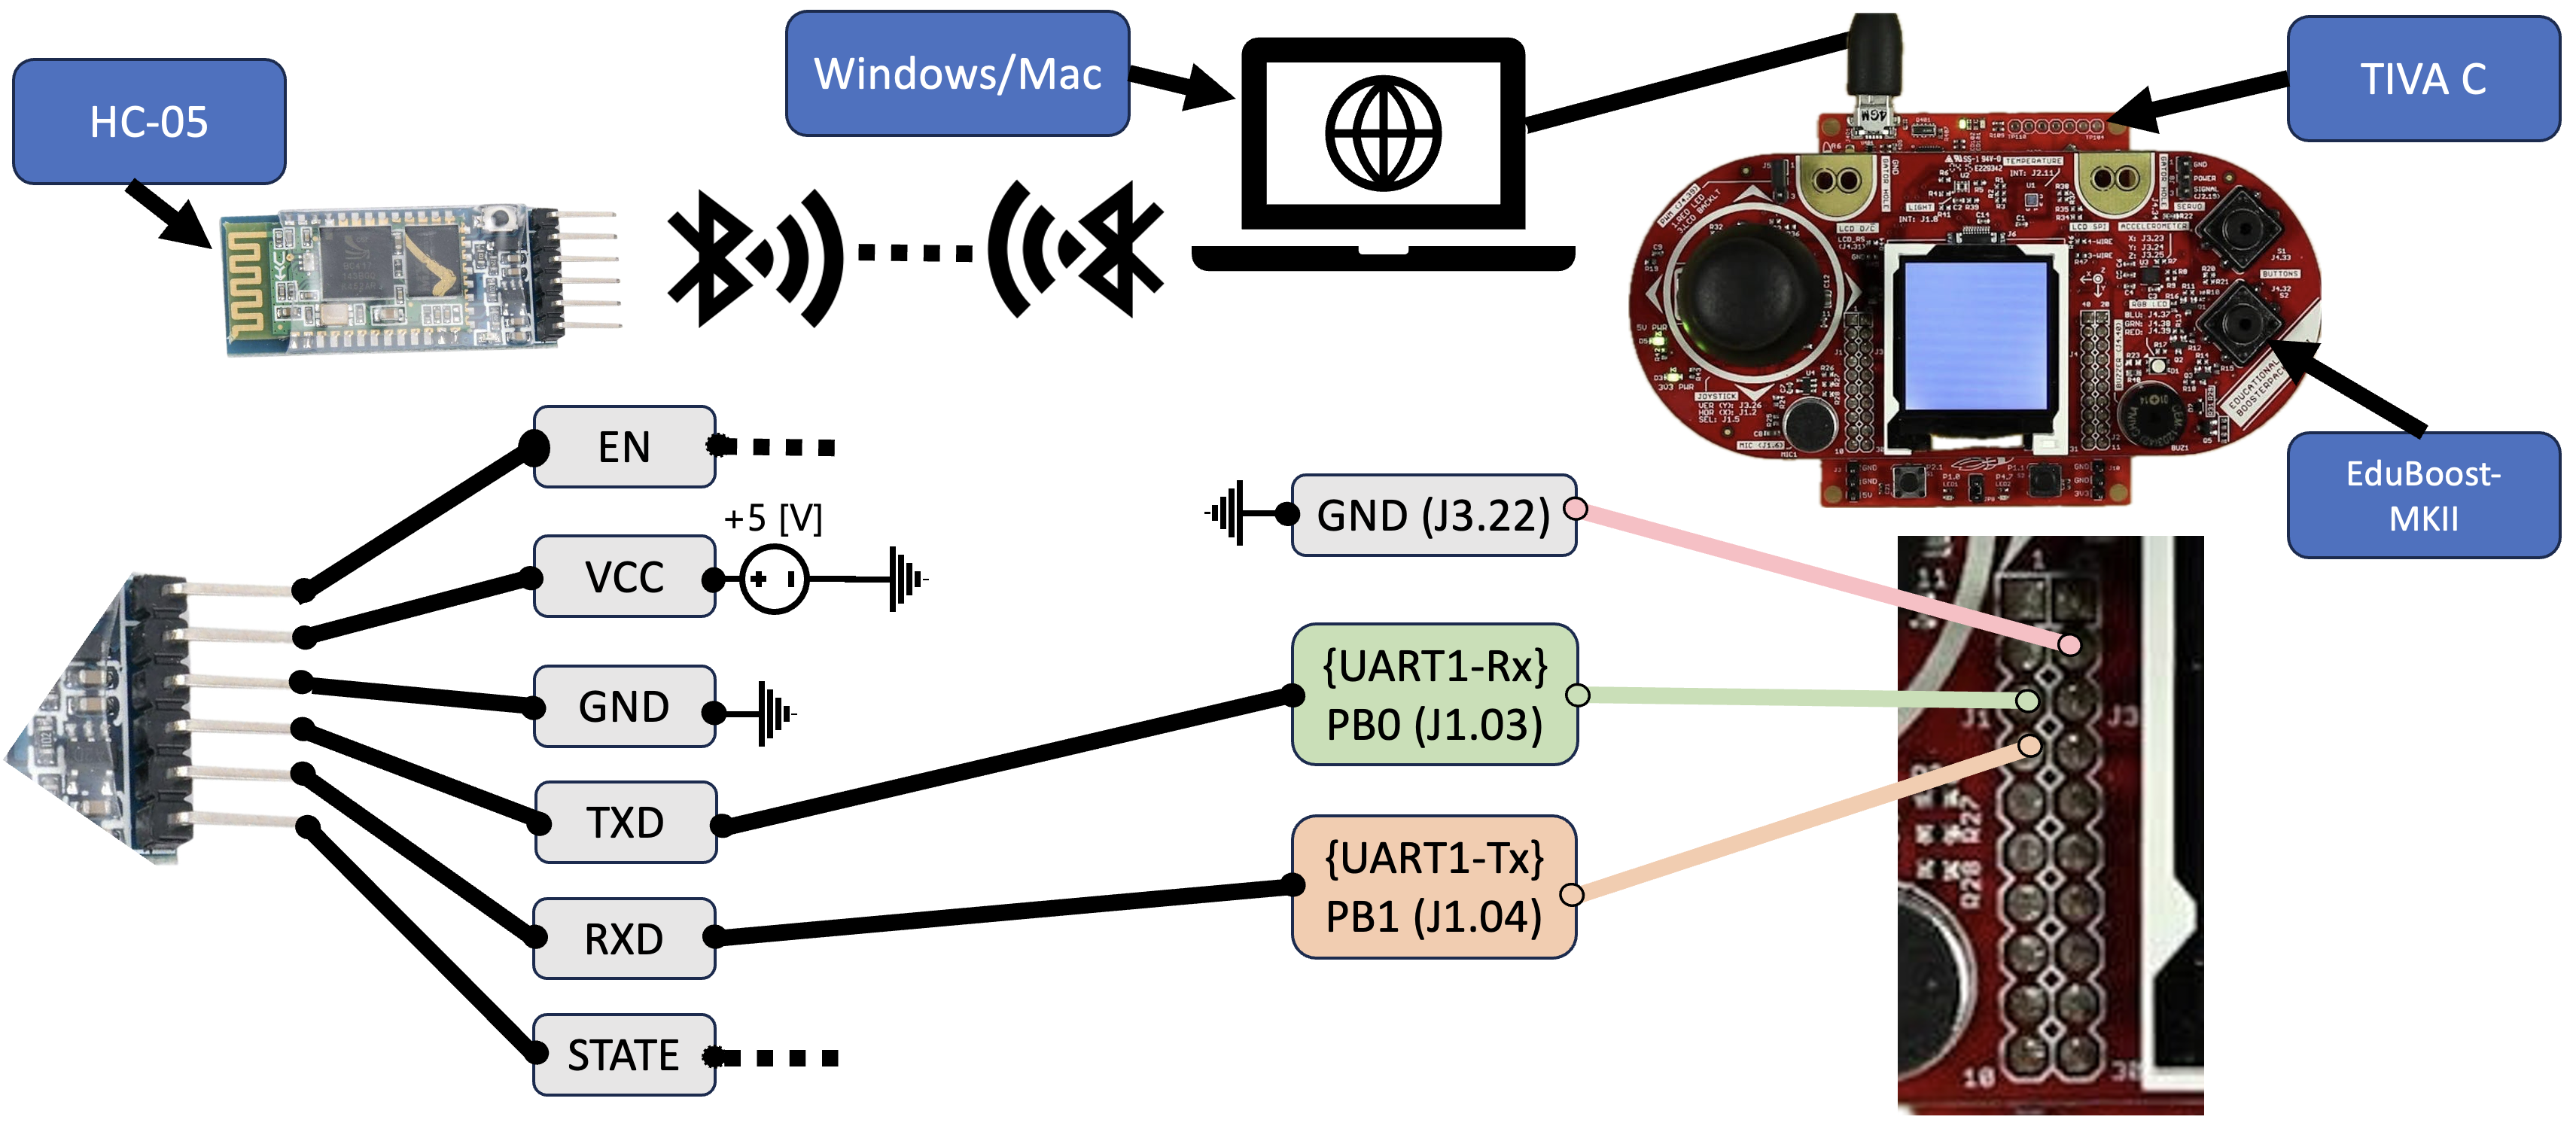
\includegraphics[width=\textwidth]{images/hardware_diagram.png} % Changed to textwidth for two columns
    \caption{High-level hardware/software partitioning.}
\label{fig:se}
\end{figure*}
\subsection{Functional Description}
The RTOS consists of one \textbf{Main} routine plus four tasks that
run in a round-robin list (Table \ref{tab:tasks}).  Main initialises
peripherals, draws axes on the LCD and starts SysTick.


\paragraph*{Task 0 – Bluetooth / Alert} polls the UART FIFO for the
ASCII value \texttt{'1'}.  On the first hit it resets \texttt{DetCount},
flags \texttt{saw=1} and chirps the buzzer; it re-chirps every 1 s as
long as detections continue.

\paragraph*{Task 1 – Microphone} samples the MKII mic, computes an RMS
window and sets \texttt{heard=1} if the level exceeds
\textit{SOUND\_THRESHOLD} ten frames in a row.

\paragraph*{Task 2 – UI} renders either the camera or microphone status
line, plus “Alarm Disabled/Armed” overlays, and handles yellow/red
detection bars.

\paragraph*{Task 3 – Buttons} debounces Button 1 (mode toggle) and
Button 2 (test-tone), and toggles the Arm/Disarm state when both are
held for one second.

\section{System Description}
\subsection{Hardware}
\begin{description}[style=nextline]
  \item[Tiva-C TM4C123GXL] 80 MHz Cortex-M4F running the RTOS.
  \item[EduBOOST-MKII] LCD, mic, push-buttons, RGB LED, buzzer.
  \item[HC-05] Classic Bluetooth module on UART1 (9600 baud).
  \item[Laptop (Win/Mac)] USB camera, Python 3.11, OpenCV 4.9.
\end{description}

\subsection{Software Development Environment}
\begin{itemize}
  \item \textbf{Embedded:} Keil µVision 5, ARM CC, Segger J-Link.
  \item \textbf{Host PC:} Python, OpenCV‐DNN, \verb|pyserial|, YOLOv4-tiny weights.
  \item \textbf{Version control:} GitHub repo \url{https://github.com/jgaucin03/MotionIoT}.
\end{itemize}

\section{RTOS Design}
The scheduler is a simple \textbf{co-operative round-robin} invoked by
\verb|SysTick_Handler| every 1 ms (1 kHz, equal quantum).  
Pre-emption occurs only at these tick boundaries; therefore we classify it
as \emph{non-preemptive round-robin}.

\subsection*{Task List}

\begin{table}[t]\centering
\caption{RTOS Task Set}\label{tab:tasks}
\begin{tabularx}{\columnwidth}{|c|c|X|}
\hline
\textbf{ID} & \textbf{Period} & \textbf{Function} \\ \hline
Task0 & 1 ms & UART/Bluetooth processing; buzzer chirp on detection \\ \hline
Task1 & 1 ms & Microphone sampling; RMS level and \texttt{heard} flag \\ \hline
Task2 & 10 ms & LCD rendering; alarm logic \\ \hline
Task3 & 5 ms & Button debounce; mode toggles \\ \hline
\end{tabularx}
\end{table}

\lstset{basicstyle=\ttfamily\footnotesize,breaklines=true}
\subsection*{Pseudo-code Excerpt (Scheduler)}
\begin{lstlisting}[language=C]
void SysTick_Handler(void){
    TCB_t *next = RunPt->next;   // round-robin list
    RunPt = next;
    (*RunPt->task)();            // cooperative switch
}
\end{lstlisting}

\section{High-Level Software Flow}
Fig.~\ref{fig:seq} details the MCU/PC interaction.

\begin{figure*}[t]
\centering
\includegraphics[width=\textwidth]{images/sequence_diagram.png}
\caption{Sequence diagram of detection → notification → LCD update.}
\label{fig:seq}
\end{figure*}

\section{Demonstration Plan}
\begin{enumerate}
  \item Laptop webcam detects a person; Python script sends ASCII ``1''.
  \item MCU chirps (\textit{Task0}) and paints yellow activity line.
  \item Cover camera: MCU clears alarm after 3 consecutive no-detection frames.
  \item Switch to microphone mode using Button 1; clap to trigger red line.
  \item Hold both buttons for 1 s to arm/disarm and show on-screen status.
\end{enumerate}

\section{Results}
\begin{itemize}
  \item End-to-end notification latency: $85\pm 7\,$ms  
        (YOLOv4-tiny $55$ ms + UART $30$ ms).
  \item System ran continuously for 30 min with no buffer overruns
        or missed UART bytes.
\end{itemize}

\section{Conclusion}
The project validates that low-cost MCUs can off-load heavyweight vision
to a host while maintaining deterministic local control via a minimal
RTOS.  Bluetooth proved adequate for indoor ranges (\textless10 m) and
simplified isolation tests.

\section{Future Work}
\begin{itemize}
  \item Integrate BLE or Wi-Fi for secure pairing and higher throughput.
  \item Migrate CNN to an edge TPU or MCU-DSP to remove laptop
        dependency.
  \item Implement pre-emptive priority scheduler for tighter audio timing.
\end{itemize}

\appendices
\section{Full Code Listing}
GitHub Key Files: \verb|tm4c/motion_detector.c| and
\verb|pc/cv.py|.

\section{Slide Deck}
\begin{figure*}[t]
\centering
\includegraphics[width=\textwidth]{presentation/ECE5436_FinalProject.pdf}
\caption{Title slide (full deck attached separately).}
\end{figure*}

% \bibliographystyle{IEEEtran}
% \bibliography{refs} % optional
\end{document}